\documentclass[]{interact}\usepackage[]{graphicx}\usepackage[]{color}
%% maxwidth is the original width if it is less than linewidth
%% otherwise use linewidth (to make sure the graphics do not exceed the margin)
\makeatletter
\def\maxwidth{ %
  \ifdim\Gin@nat@width>\linewidth
    \linewidth
  \else
    \Gin@nat@width
  \fi
}
\makeatother

\definecolor{fgcolor}{rgb}{0.345, 0.345, 0.345}
\newcommand{\hlnum}[1]{\textcolor[rgb]{0.686,0.059,0.569}{#1}}%
\newcommand{\hlstr}[1]{\textcolor[rgb]{0.192,0.494,0.8}{#1}}%
\newcommand{\hlcom}[1]{\textcolor[rgb]{0.678,0.584,0.686}{\textit{#1}}}%
\newcommand{\hlopt}[1]{\textcolor[rgb]{0,0,0}{#1}}%
\newcommand{\hlstd}[1]{\textcolor[rgb]{0.345,0.345,0.345}{#1}}%
\newcommand{\hlkwa}[1]{\textcolor[rgb]{0.161,0.373,0.58}{\textbf{#1}}}%
\newcommand{\hlkwb}[1]{\textcolor[rgb]{0.69,0.353,0.396}{#1}}%
\newcommand{\hlkwc}[1]{\textcolor[rgb]{0.333,0.667,0.333}{#1}}%
\newcommand{\hlkwd}[1]{\textcolor[rgb]{0.737,0.353,0.396}{\textbf{#1}}}%
\let\hlipl\hlkwb

\usepackage{framed}
\makeatletter
\newenvironment{kframe}{%
 \def\at@end@of@kframe{}%
 \ifinner\ifhmode%
  \def\at@end@of@kframe{\end{minipage}}%
  \begin{minipage}{\columnwidth}%
 \fi\fi%
 \def\FrameCommand##1{\hskip\@totalleftmargin \hskip-\fboxsep
 \colorbox{shadecolor}{##1}\hskip-\fboxsep
     % There is no \\@totalrightmargin, so:
     \hskip-\linewidth \hskip-\@totalleftmargin \hskip\columnwidth}%
 \MakeFramed {\advance\hsize-\width
   \@totalleftmargin\z@ \linewidth\hsize
   \@setminipage}}%
 {\par\unskip\endMakeFramed%
 \at@end@of@kframe}
\makeatother

\definecolor{shadecolor}{rgb}{.97, .97, .97}
\definecolor{messagecolor}{rgb}{0, 0, 0}
\definecolor{warningcolor}{rgb}{1, 0, 1}
\definecolor{errorcolor}{rgb}{1, 0, 0}
\newenvironment{knitrout}{}{} % an empty environment to be redefined in TeX

\usepackage{alltt}

% \usepackage{lineno,hyperref}
% \modulolinenumbers[5]

\usepackage{multirow}
\usepackage{color,soul}
\usepackage{array}
\newcolumntype{L}[1]{>{\raggedright\let\newline\\\arraybackslash\hspace{0pt}}m{#1}}
% \usepackage{caption}

\usepackage[none]{hyphenat} % to cancel auto-hyphenation

\usepackage[numbers,sort&compress]{natbib} % for reference/citation formating
\bibpunct[, ]{[}{]}{,}{n}{,}{,}
\renewcommand\bibfont{\fontsize{10}{12}\selectfont}
\IfFileExists{upquote.sty}{\usepackage{upquote}}{}
\begin{document}

% puts R2 in bold in table 3
\makeatletter
\DeclareRobustCommand\bfseries{%
  \not@math@alphabet\bfseries\mathbf
  \fontseries\bfdefault\selectfont
  \boldmath % <-- added
}
\makeatother

\makeatletter % for spacing figures at the end of the document
\@fpsep\textheight
\makeatother




\title{Survival Analysis of Questions Posted on the iFixit Answers Forum}

\author{
\name{Lisa Oshita\textsuperscript{a}\thanks{CONTACT Lisa Oshita Email: l.oshita@yahoo.com}, Anthony Pileggi\textsuperscript{b}, Shannon Pileggi\textsuperscript{a}}
\affil{\textsuperscript{a}Department of Statistics, California Polytechnic State University, CA, 93407; \textsuperscript{b}iFixit, 1330 Monterey St, San Luis Obispo, CA 93401, United States}
}

\maketitle

\begin{abstract} 
iFixit's community-driven online question and answer forum (CQA), \textit{Answers}, provides a platform for thousands of users to ask and answer questions related specifically to device repair. This paper presents a survival analysis of the time until a question posted on iFixit's \textit{Answers} forum receives it's first response. A Cox proportional hazards model was developed to identify variables associated with response time. Though several predictors were significant, the model's predictive accuracy was low ($R^2 = 0.15$). Significant predictors included the device category of the question (questions pertaining to Apple products received answers faster than others (HR = 2.54, 95\% CI = (2.32, 2.79)), factors related to the question's title (e.g., if it was phrased as a question (HR = 1.29, 95\% CI = (1.21, 1.38))), and the day of the week the question was posted (questions posted over the weekend received answers slower than those posted on a weekday (HR = 0.87, 95\% CI = (0.82, 0.93))). Future studies can investigate whether factors identified as significant in this analysis can be generalized to other CQAs.
\end{abstract}

\begin{keywords}
Cox regression; CQA forum; response time; survival analysis; survival probabilty 
\end{keywords}


\section{Introduction}

Founded in 2003, iFixit teaches thousands of users across the globe how to fix their own broken devices. This company provides over 40,000 free online repair guides and hosts a CQA, the \textit{Answers} forum, featuring questions pertaining to over 11,000 devices with over 130,000 user-posted solutions. One critical key feature of CQAs like \textit{Answers} is question response times. Fast response times have been shown to be associated with positive user experience and increased web traffic---factors that are extremely valuable to the reputation and longevity of the CQA \cite{Rechavi2011}. Analysis of response times can reveal factors that affect how quickly questions receive answers, which can lead to suggestions for how users can ask questions to minimize response times and for how forum design can be improved.

However, analysis and prediction of response times on CQAs have not been thoroughly investigated. There is need for further analysis in this area, as the majority of existing research focuses on assessing and predicting question or answer quality. This paper presents a survival analysis on the time until a question receives its first answer on iFixit's \textit{Answers} forum, in order to determine factors significantly related to response time and to predict survival probabilities of questions.


\section{Related Work}

With the recent increase in the popularity and use of CQAs, these data-rich platforms have been the subject of a multitude of studies. Regarding analysis of response times, \cite{Bhat2014} developed a classification model using both textual and non-textual features to estimate response times for questions posted on \textit{Stack Overflow}. \cite{Mahmud2013} used parametric methods and proposed models to predict response times based on exponential distributions. \cite{Asaduzzaman2013} instead focused exclusively on unanswered questions and created a model to predict how long a question would remain unanswered. However, all research mentioned restricted analysis to either questions for which response times were observed or to questions that remained unanswered. The research presented in this paper uses survival analysis, a method not yet applied to CQAs, to allow for analysis of both answered and unanswered questions in a unified framework. 

The majority of existing research has been focused on predicting question and answer quality. \cite{Weimer2007} developed a classification algorithm to assess the quality of posts on \textit{Nabble.com} using primarily textual features of questions. \cite{Blumenstock2008} also determined that textual features (e.g. word count) was the most accurate predictor of Wikipedia article quality (Wikipedia articles can represent the same kind of user-generated content featured on CQAs). \cite{Fu2015} instead found that non-textual features, like revision and comment count or the number of points a user has, were the most useful indicators of quality. A number of other studies have also developed classification algorithms using textual and non-textual features with the similar goal of predicting question or answer quality \cite{Yao2015, Toba2014, Ponzanelli2014a, Ravi2014}. The present analysis seeks to utilize both textual and non-textual features of questions on iFixit's \textit{Answers} forum to investigate if factors that indicate that a question is of high quality also lead to faster response times.


\section{Materials}

The data analyzed contained 8,025 questions posted from April 8, 2017 to July 7, 2017 (date of data download). Variables in the data included: device name, device category, question title, text, tags, new user status, date and time the question was posted, and date and time the first answer was received. Variables derived can be found in Table \ref{table:1}. The Appendix contains details on variable derivation, as well as an example of an answered and unanswered question in Table \ref{table:5}. 


\section{Methods}

Questions analyzed were restricted to those posted in English. Time until event was defined as the time since posting until a question received its first answer. For questions that did not receive an answer by the download date, time until event values were defined as the time since posting to the time the data was downloaded. Such questions were considered right-censored, meaning that exact answer times for these questions are greater than the observed download time (questions may receive answers after the download date) \cite{Kleinbaum2011}. 

Survival was defined as the event that a question did not receive an answer beyond a certain time, \textit{t}. Estimates of survival probability were generated with the Kaplan-Meier method, which adjusts to the presence of right-censored observations, or unanswered questions \cite{Bland1998}. From these estimates, survival curves were constructed to examine the overall question survival experience. Mean and median survival times were also computed. 

As the probability distribution for response times is unknown, a non-parametric Cox proportional hazards model was developed to predict question survival probability \cite{Moore2010}. To build the model, the full data was partitioned into five separate sets \cite{Rodriguez2010}. Univariate analysis, performed on one training set, was used to identify variables to include in the final predictive Cox model \cite{Hammermeister1979}. For this process, each predictor was entered into univariate Cox models and evidence of association with response times was assessed. Those with partial likelihood ratio p-values of less than 0.001 were included in the final model. Transformations and restricted cubic splines were also explored through a similar process. The combination of which transformation, square root or log-transformed, and restricted cubic spline with three, four, or five knots, were selected for each continuous predictor based on the AIC statistic \cite{Harrell2015}. All significant categorical and continuous predictors, in final form, were included in the model for five-fold cross-validation. 

In each iteration of cross-validation, the full model was built on the training set and used to compute predicted hazard ratios on the corresponding test set. To assess performance, predicted hazard ratios were entered into separate Cox models as the single quantitative predictor with response times as survival time. The resulting Nagelkerke's $R^2$ statistic, concordance statistic, Somers' \textit{Dxy}, partial likelihood ratio and p-value, were assessed as indicators of the model's performance \cite{Chen}. The partial likelihood ratio is a ratio of the log partial likelihood function evaluated at the parameter estimates, equivalent to a goodness of fit measure of the model with predictors, and the log partial likelihood function for the null model without predictors and only the baseline hazard function, equivalent to a goodness of fit measure for the null model. The p-value for this statistic was calculated from the $\chi^2$ distribution \cite{Oakes1981}. Concordance statistics and Somers' \textit{Dxy} are a measure of the model's discriminative ability. Concordance is defined as the probability that for any two randomly chosen questions, the question with the shorter response time also has the higher predicted hazard. Concordance statistics close to 1 indicate high discriminative ability, while statistics close to 0.5 indicate discordance, or random predictions. Somers' \textit{Dxy} is the difference between the model's concordance statistic and discordance, 0.5. A Somers' \textit{Dxy} statistic of 0 indicates random predictions, while a statistic equal to 1 indicates perfect predictions \cite{Harrell2015}. These metrics were computed for each iteration on every training and test set. Averages of metrics across training and test sets were evaluated. The final model was then fit to the full data and the same metrics were computed and compared. 

Correlations between scaled Schoenfeld residuals, differences between observed and expected predictor values for questions that received answers, and a function of time, were examined to assess the proportional hazards assumption that the effect of predictors on hazard does not depend on time \cite{Grambsch1994}. Significant correlations would indicate a predictor has violated this assumption.

All computation was executed under \texttt{R} version 3.4.3.  Kaplan-Meier estimates of survival probability were computed with the \texttt{Surv} and \texttt{survfit} functions of the \texttt{Survival} package in R. To compute predicted survival probabilities using the final model, the \texttt{predictSurvProb} function was used from the \texttt{pec} package. This function uses the Cox model and a vector of times to compute predictions. Data used for this analysis was published on Mendeley Data (DOI: 10.17632/shfkj785yb.1). Code for variable setup and analysis is available upon request. 


\section{Results}



% Distribution of answer times
% \begin{figure}[!htbp]
%   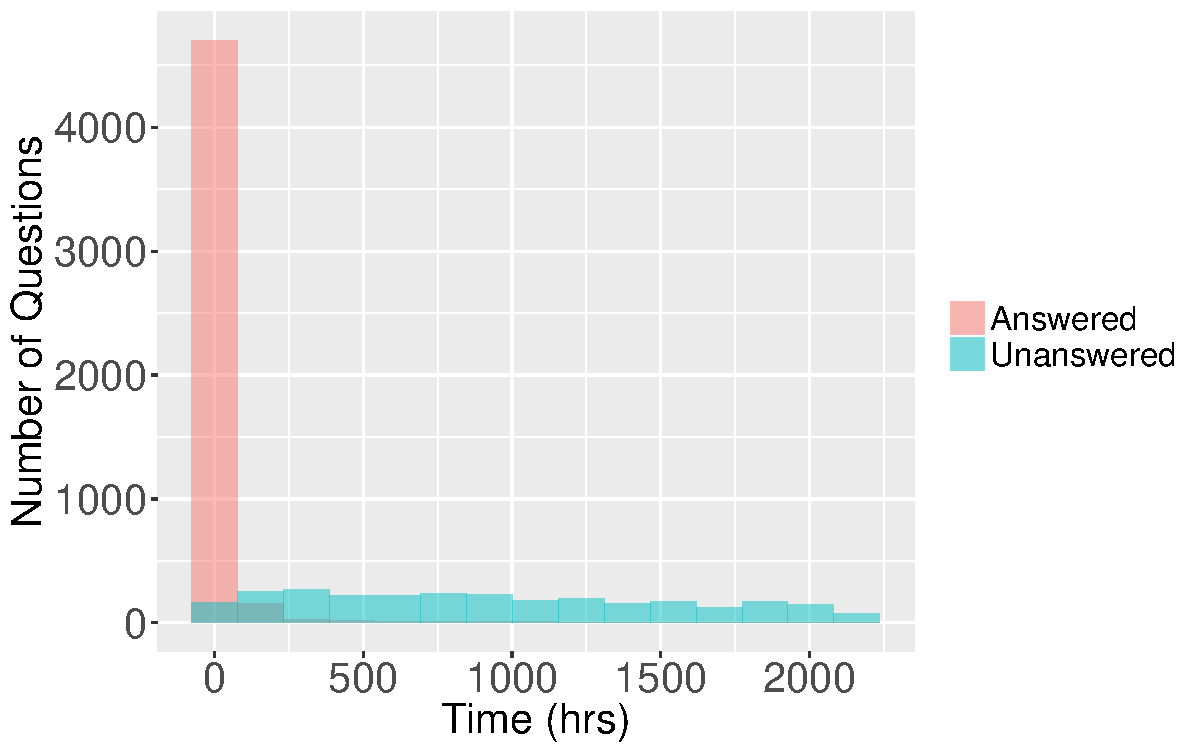
\includegraphics[scale=0.5]{FIG1.pdf}
%   \label{fig:1}
% \end{figure}
% 
% % Kaplan-Meier curve
% \begin{figure}[!htbp]
%   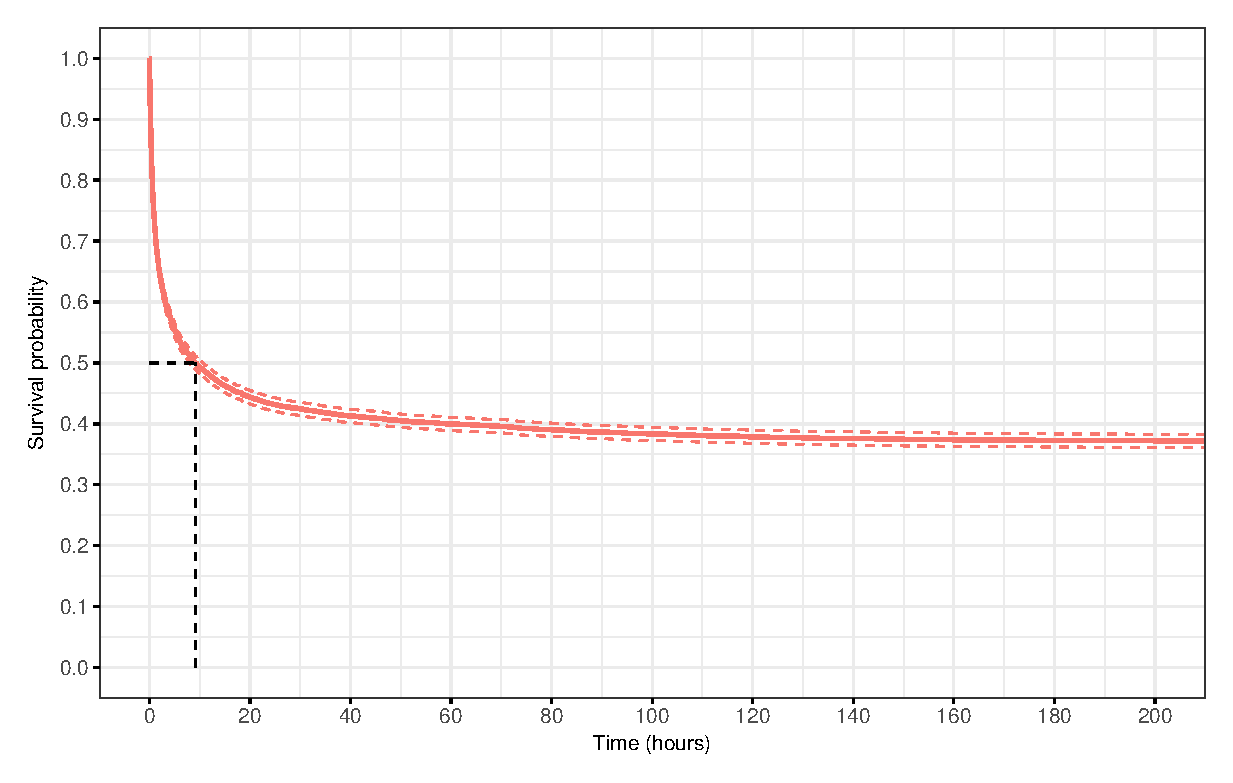
\includegraphics[scale=0.5]{FIG2.eps}
%   \label{fig:2}
% \end{figure}

  Of 8,025 questions in the full data, 7,760 were in English (97\% of the full data). Of those questions, 4,951 (63.8\%) received an answer by the download date. The shortest response time was 0.5 hours. The longest was 2,159 hours (90 days). Figure 1 shows the distribution of response times for all questions analyzed. 



Figure 2 shows the Kaplan-Meier estimated survival probability curve for all questions in the data. The curve indicates that if a question does not receive an answer soon after it is posted, the likelihood of it receiving an answer in the future is low. The Kaplan-Meier estimated mean survival time, or the average time until a question received its first answer was 776 hours, or 32.3 days. The median survival time, the time at which 50\% of the questions in the data received an answer, was 9.2 hours.




Each training set contained 6,208 questions; each test set contained 1,552 questions. Univariate analysis performed on one training set indicated that all categorical predictors were significant with partial likelihood ratio p-values of less than 0.001. Continuous predictors, excluding device length and average tag length, also resulted in univariate p-values of less than 0.001. Applying either square root or log transformations to all continuous predictors resulted in univariate p-values of less than 0.001. For variables that contained zeros, one was added to each observation before applying the log transformation. The following transformations were applied to continuous variables: square root transformation of average tag frequency, log plus one transformation of average tag length, log plus one transformation of device name length, square root transformation of line break to text length ratio, and log transformation of text length. All categorical predictors and all continuous predictors with necessary transformations were retained for the full model. 

Table \ref{table:2} shows the results of determining the optimal number of knots for each continuous predictor. Those marked with an asterisk (*) were included in the final model. 

Average performance metrics for test and training sets are in Table \ref{table:3}. Partial likelihood ratios and p-values indicate that the model as a whole is significantly associated with response time. However, $R^2$ statistics and discrimination indexes are considerably low. Metrics for the final model's performance on the full data, also found in Table \ref{table:3}, are consistent with metrics found in cross-validation and indicate low predictive accuracy. Results for training, test, and the full data did not change significantly, indicating that the model was not over fit. 



Assessing the proportional hazards assumption indicated that several levels of the device categorization variable, specifically Apple Product, Camera, Game Console, and Other, violated the assumption. 

As a whole, the final model was significant with a partial likelihood ratio of 1265.29 (p-value \textless0.0001). Its $R^2$ statistic was 0.15, and Somers' \textit{Dxy} was 0.27. 

The following are interpretations of select hazard coefficients in Table \ref{table:4}. Hazard is approximately equivalent to the conditional probability that a question will receive an answer within the next moment in time, given that it has not already received an answer. 




\begin{itemize}
  \item The estimated hazard of receiving an answer is 154\% higher (95\% CI (132\%, 179\%)) for questions pertaining to Apple products than the hazard for questions about Android and Other phones, controlling for all other predictors.
  \item The estimated hazard of receiving an answer is 25\% lower (95\% CI (19\%, 29\%)) for questions with titles that contain at least one word considered to be frequently-used among unanswered questions, than the hazard for questions with titles that do not, controlling for all other predictors. 
  \item The estimated hazard of receiving an answer for questions posted on a weekend is 13\% lower (95\% CI (7\%, 18\%)) than the hazard for questions posted on a weekday, controlling for all other predictors.
\end{itemize}


\section{Discussion}

Results and coefficients of the final model reveal how users can ask questions in order to decrease response time. Findings suggest that users should phrase the title in the form of a question, use correct grammar (e.g. punctuation and capitalization), include specific and concise tags, and post the question on a weekday. 

% Predictors found to be significant included: device category, if the question was posted on a weekend or a weekday, whether or not the question's title contained at least one word considered frequently-used among unanswered questions, and whether or not the question's title ends in a question mark. 

The model's weak predictive accuracy, which may be explained by limitations in the data, lead to suggestions for changes in CQA design. Many users incorrectly specified the device name (e.g. a user asking a question about a Turtle Beach Ear Force XO ONE headset defined the device name as, ``Turtle Beach Ear Force Xmy grandson chewed through the wire while he was playing it's brand-new is there anyway I can have it fixed0 One''), or did not include a device name. Many users also incorrectly used the tagging system by including ambiguous and lengthy tags like ``someone sat on it :('' or ``help me please!!!!!'' (tags are generally a couple key words that allow the answering community to quickly discern the question's topic). It is likely that these inconsistencies contributed to the final model's low predictive power. This, along with the results of the final model, reveal some of the ways the CQA can be structured to potentially decrease response times. As findings indicate that questions with correctly defined tags and device names may lead to quicker response times, the CQA can provide a stricter framework for asking questions. Allowing users to enter any device name or tag leaves room for user error, shown by the examples described above. Instead, the CQA can restrict the tags or devices that users can include to a drop-down list. The CQA can also include more tips to guide users asking questions. Implementing a more structured framework for asking questions can help users create understandable and clear questions and in turn decrease response times, as well as create a set of consistent questions for improved analysis. 

% \section{Vitae}
% 
% Lisa Oshita is a senior undergraduate statistics major at the California Polytechnic State University in San Luis Obispo. Shannon Pileggi is an Assistant Professor in the Statistics Department at California Polytechnic State University, San Luis Obispo. Anthony Pileggi is a Data Scientist at iFixit. Declarations of interest: none. 

% \section{Author Contributions}
% 
% All authors contributed to the analysis featured in this paper and have edited and approved of the final article. 

\section*{Acknowledgements}

 We would like to thank iFixit for providing access to the CQA data.
 
\section*{Disclosure Statement}

We wish to confirm that there are no known conflicts of interest associated with this publication.

\section*{Funding}
 
This research was supported by the Bill and Linda Frost fund of the California Polytechnic State University of San Luis Obispo. This sponsor was not involved in any aspect of this paper's analysis.


\bibliographystyle{tfs}
\bibliography{references}


\section{Appendices}

\appendix

\section{Posted questions}

Table \ref{table:5} provides observed and derived variable values from an example of an answered question (regarding the iPhone 6) and unanswered question (regarding android tablet). All fields in device, title, text, and tags are shown as the users entered it. 


\section{Variable Derivation}

\subsection{Average tag frequency}

This variable was created to investigate if including popular or widely-used tags in a question can lead to faster response times, based off of findings from \cite{Bhat2014}. This was computed as the average frequency, or proportion of times a question's tags appear in all of the data set. Questions without tags were assigned a value of 0.  If a question has a higher average, then at least one of its tags are considered frequently-used.


\subsection{Average tag length}

This variable was created to investigate if questions with correctly defined tags have faster response times than questions that do not include tags or incorrectly use the tagging system. It is hypothesized that questions with ambiguous or lengthy tags make it difficult for the answering community to discern the question's topic, and thus have slower response times or remain unanswered. 


\subsection{Device categorization}

Original device categories defined by iFixit included: Apparel, Appliance, Camera, Car and Truck, Computer Hardware, Electronics, Game Console, Household, Mac, Media Player, PC, Phone, Skills, Tablet, Vehicle. Device titles were parsed and certain categories were combined or separated to create a new device categorization variable to use in the Cox model. Final categories created included: Android/Other Phone, Apple Product, Camera, Electronics, Game Console, Home, Other, PC, Tablet, Vehicle. Under the original device categorization, 1,954 questions (25.2\% of 7,760) were categorized incorrectly and indicated an NA for its category. Missing values were a result of users creating questions for devices not already in the iFixit's database, or from the user incorrectly defining the device name. For questions with missing categories, key words were searched for in device titles to re-categorize accordingly. All other questions with ambiguous device titles were categorized as Other. 


\subsection{Device name length}

This variable was created to investigate if questions with correctly defined device names have faster response times than questions that do not include a name or are incorrectly defined. Similar to the average tag length variable, it is hypothesized that questions with incorrectly defined device names (often lengthy) make it difficult for the answering community to discern the question's topic, and thus have slower response times. 


\subsection{If the question's text contains end punctuation}

This variable was created to investigate if sentences with no end punctuation take longer to receive an answer.


\subsection{If the question's title contains terms considered frequently-used among answered/unanswered questions}

These variables were created to investigate if questions pertaining to popular topics receive answers faster than questions that do not. Similarly, another variable was created to investigate if questions pertaining to unpopular topics receive answers slower than questions that do not. This variable was created based off of methods from \cite{Correa2013} and \cite{Ravi2014}.

To create the variables, the data was separated between answered and unanswered questions. For the data frame containing answered questions, text mining techniques were used to create a list of every word within each questions' titles and the proportion of times those words occurred among all answered questions' titles, defined as the frequency. The same was performed for the data frame containing unanswered questions. ``Frequently-used'' words in answered questions were defined as those that appeared in 1\% or more of all answered questions' titles, and appeared in more answered questions than in unanswered questions. To determine the latter, a ratio of frequencies was assessed. The ratio was calculated as the proportion of times a word occurred among answered questions, to the proportion of times a word occurred in unanswered questions. As an example, if ``cracked'' appeared in 2\% of answered questions and 0.1\% of unanswered questions, it would be considered ``frequently-used'' among answered questions as it occurs in more than 1\% of answered questions' titles and occurs 20 times more in answered question than in unanswered questions (ratio = 0.02/0.001 = 20). Similarly, ``frequently-used'' words in unanswered questions must occur in 1\% or more of all unanswered question's titles and occur in more unanswered questions than answered questions. As there was some overlap between ``frequently-used'' words in each list and levels of the device categorization variable, every word that matched a device name was removed from the lists. Table \ref{table:6} contains the resulting terms for answered questions (111 words) and for unanswered questions (32 words).

\subsection{If the question's title ends in a question mark}

This variable was created to investigate if questions with titles in the form of questions receive answers faster than those otherwise phrased \cite{Bhat2014}. 


\subsection{If the user made an effort to solve the problem prior to asking the question}

This variable indicates true if the asker included words in the question's text that indicate that the user made prior effort to find the solution before posting. Words searched for include: tried, searched, researched, tested, replaced, used, checked, investigated, considered, measured, attempted, inspected, fitted. This variable was created based off of findings and methods from \cite{Bhat2014} and \cite{Harper2008}. 


\subsection{Line break to text length ratio}

This variable was created to investigate if questions that include line breaks in the text are easier to read than questions that do not include any, and thus have shorter response times. Questions with a ratio of 0 tend to include either short, ambiguous texts (e.g. "Start button not working.") or long and lengthy texts, and tend to remain unanswered or have slower response times. Questions with a ratio of greater than 0 tend to have faster response times. 


\section{Tables}

% Table of derived predictors
\begin{table}[p]%[!htbp]
\tbl{Categorical and continuous variables derived}
% \centering
{\begin{tabular}{|L{2cm}|L{10cm}|}
  \hline
  \multirow{9}{2cm}{\textbf{Categorical Variables}} & Device category the question pertains to. Categories include: Android/Other Phone, Apple Products, Camera, Electronics, Game Console, Home, Other, PC, Tablet, Vehicle \\ \cline{2-2}
  & If the question was posted on a weekend or on a weekday \\ \cline{2-2}
  & If the question's text contains end punctuation marks (. ? !) \\ \cline{2-2}
  & If the question's text is in all lower case \\ \cline{2-2}
  & If the question's title contains at least one word considered to be ``frequently-used'' among answered questions \\ \cline{2-2}
  & If the question's title contains at least one word considered to be ``frequently-used'' among unanswered question \\ \cline{2-2}
  & If the question's title ends in a question mark \\ \cline{2-2}
  & If the user edited or added information to the question's text after posting it \\ \cline{2-2}
  & If the user made an effort to solve the problem prior to asking the question \\ \hline
  \multirow{5}{2cm}{\textbf{Continuous Variables}} & Average number of characters in each question's tags (average tag length)\\ \cline{2-2}
  & Average frequency for all of a question's tags (average tag frequency) \\ \cline{2-2}
  & Number of characters in the question's text (text length) \\ \cline{2-2}
  & Number of characters in the user-defined device name (device name length) \\ \cline{2-2}
  & Ratio of the number of line breaks to the number of characters in the question's text (line break to text length ratio) \\ \hline
\end{tabular}}
% \caption{Categorical and continuous variables derived}
\label{table:1}
\end{table}


% Splines Square root transformation of the average tag frequency
\begin{table}[p]% [!htbp]
% \centering
\tbl{The model with the lowest AIC was used to determine the optimal k number of splines for each continuous predictor.} 
{\begin{tabular}{| L{5cm} | l | l |}
  \hline
  \textbf{Predictor} & \textbf{K} & \textbf{AIC} \\ 
  \hline
  \multirow{4}{5 cm}{$\sqrt{\textnormal{average tag frequency}}$} 
  & 0\textbf{*} & 65890.75 \\ 
  & 5 & 65891.69 \\ 
  & 4 & 65891.75 \\ 
  & 3 & 65892.35 \\ 
  \hline
  \multirow{4}{5 cm}{$\log\left({\textnormal{average tag length} + 1}\right)$}
  & 0 & 65920.24 \\ 
  & 5 & 65911.20 \\ 
  & 4\textbf{*} & 65910.81 \\ 
  & 3 & 65914.98 \\ 
  \hline
  \multirow{4}{5 cm}{$\log\left({\textnormal{device length} + 1}\right)$}
  & 0 & 65918.06 \\ 
  & 5\textbf{*} & 65847.34 \\ 
  & 4 & 65880.89 \\ 
  & 3 & 65898.00 \\ 
  \hline
  \multirow{4}{5 cm}{$\sqrt{\textnormal{line breaks / text length}}$}
  & 0 & 65890.28 \\ 
  & 5 & 65884.70 \\ 
  & 4 & 65882.98 \\ 
  & 3\textbf{*} & 65881.93 \\ 
  \hline
  \multirow{4}{5cm}{$\log\left({\textnormal{text length}}\right)$} 
  & 0 & 65862.83 \\ 
  & 5\textbf{*} & 65862.02 \\ 
  & 4 & 65863.35 \\ 
  & 3 & 65862.08 \\ 
  \hline
\end{tabular}}
\label{table:2}
\end{table}

% Cross-validation metrics
\begin{table}[p]%[!htbp]
% \centering
\tbl{Performance metrics of final model. (HR: Hazard Ratio, LR: Partial Likelihood Ratio)}
{\begin{tabular}{|r|r|r|r|r|r|r|r|}
  \hline
 & \textbf{HR} & \textbf{LR} & \textbf{p-value} & \textbf{$R^2$} & \textbf{\textit{Dxy}} & \textbf{Concordance} \\ 
  \hline
  \textbf{Training Sets} & 2.03 & 937.39  & \textless0.0001 & 0.14 & 0.27 & 0.63 \\ 
  \textbf{Test Sets}     & 1.99 & 220.83  & \textless0.0001 & 0.14 & 0.26 & 0.63 \\
  \textbf{Full Data}     & 2.03 & 1165.03 & \textless0.0001 & 0.14 & 0.28 & 0.63 \\ 
   \hline
\end{tabular}}
\label{table:3}
\end{table}

% Final model on full data
\begin{table}[p]%[!htbp]
% \centering
\tbl{Coefficients for predictors in the final model. (Continuous predictors fit with restricted cubic splines are not shown)} 
{\begin{tabular}{|l L{5.5cm}|c|c|}
  \hline
 \textbf{Variable} & & \textbf{Coefficient (SE)} & \textbf{p-value} \\ \hline
  Device Category & Apple Product & 0.93 (0.048) & \textless0.0001 \\ 
                  & Camera & -0.32 (0.090) & \\ 
                  & Electronics & -0.01 (0.078)  & \\ 
                  & Game Console & 0.24 (0.083)  & \\ 
                  & Home & 0.34 (0.070) &  \\ 
                  & Other & -0.13 (0.056)  & \\ 
                  & PC & 0.28 (0.060) &  \\ 
                  & Tablet & -0.16 (0.081)  & \\ 
                  & Vehicle & 0.40 (0.069)  & \\
                  & Android/Other Phone (reference) & --- & \\ \hline
  \multicolumn{2}{|l|}{Weekend} & -0.13 (0.033)  & \textless0.0001 \\ \hline
  \multicolumn{2}{|l|}{Text contains end punctuation} & 0.03 (0.050) & 0.613 \\ \hline
  \multicolumn{2}{|l|}{Text is in all lower case} & -0.18 (0.064) &  0.006 \\ \hline
  \multicolumn{2}{|L{9cm}|}{Title contains terms considered frequently-used among answered questions} & 0.05 (0.042) &  0.260 \\ \hline
  \multicolumn{2}{|L{9cm}|}{Title contains terms considered frequently-used among unanswered questions} & -0.28 (0.034)  & \textless0.0001 \\ \hline
  \multicolumn{2}{|L{9cm}|}{Title ends in a question mark} & 0.26 (0.033) &  \textless0.0001 \\ \hline
  \multicolumn{2}{|L{9cm}|}{User edited or added to the question's text after posting it} & 0.30 (0.086)  & 0.001 \\ \hline
  \multicolumn{2}{|L{9cm}|}{User was a member for less than one day before posting} & -0.11 (0.036)  & 0.003 \\ \hline
  \multicolumn{2}{|L{9cm}|}{User made an effort to solve the problem prior to asking the question} & -0.07 (0.036)  & 0.045 \\ \hline
  \multicolumn{2}{|L{9cm}|}{Square root of the average tag frequency} & 2.23 (0.720)  & 0.002 \\ \hline
\end{tabular}}
\label{table:4}
\end{table}

\begin{table}[p]%[!htbp]
% \centering
\tbl{Examples of an answered question (left) and an unanswered question (right)}
{\begin{tabular}{|L{4cm}|L{5cm}|L{5cm}|}
\hline
\textbf{Device} & iPhone 6 & android tablet \\ \hline
\textbf{Title} & iPhone water damage, touch screen issue & ccccaaaan you help me fix my touch screen \\ \hline
\textbf{Text} & So I dropped my iPhone in water 4 days ago. Have done the whole rice thing and seen huge difference in it. However, only one side of my screen works and it is the one side which I need to unlock the phone. What would be the best way forward? & touch screen not worki\\ \hline
\textbf{Tags} & touchscreen, water damage & NA\\ \hline
\textbf{Response Time (hrs)} & 1.361 & NA \\ \hline 
\textbf{Device Category} & Apple Product & Tablet \\ \hline
\textbf{Day Posted} & Weekday & Weekday \\ \hline
\textbf{Text length (characters)} & 241 & 81 \\ \hline
\textbf{Device name length (characters)} & 8 & 18\\ \hline
\textbf{Average tag length (characters)} & 11.5 & 47 \\ \hline
\textbf{Average tag frequency} & 0.0097 & 0 \\ \hline
\textbf{Text contain end punctuation?} & True & False \\ \hline
\textbf{Text in all lower case?} & False & True \\ \hline
\textbf{Title end in a question mark?} & False & False \\ \hline
\textbf{Line break to text length ratio} & 0 & 0 \\ \hline
\textbf{User indicate prior effort?} & False & False \\ \hline
\textbf{User update question after posting?} & False & False \\ \hline
\textbf{Frequently-used answered words?} & True & True \\ \hline
\textbf{Frequently-used unanswered words?} & False & False \\ \hline
\end{tabular}}
\label{table:5}
\end{table}

% Table with list of frequently-used words
\begin{table}[p]%[!htbp]
% \centering
\tbl{Frequently-used terms among answered and unanswered questions' titles, ordered by decreasing frequency}
{\begin{tabular}{|L{4cm}|L{8cm}|}
  \hline
 \textbf{Frequently-used terms among answered questions} & screen, turn, working, replacement, power, work, replace, charging, charge, button, touch, black, turning, broken, start, stuck, new, LCD, upgrade, problem, change, port, replaced, card, open, boot, replacing, remove, reset, back, drive, error, cable, ssd, cracked, hard, one, dropped, logic, lines, white, keeps, pro, dead, now, front, damage, switch, parts, glass, still, charger, issue, sim, turns, digitizer, just, mode, model, backlight, usb, stopped, logo, starting, know, unresponsive, password, factory, call, use, damaged, find, sensor, possible, fixed, side, galaxy, data, ipod, problems, issue, slow, system, connector, without, overheating, code, ram, air, microphone, please, red, much, plugged, getting, booting, left, way, buy, plus, time, loose, lock, coming, got, shuts, says, install, key, door, top \\
  \hline
  \textbf{Frequently-used terms among unanswered questions} & sound, light, wifi, speaker, connect, picture, stay, noise, bluetooth, isnt, apps, going, rear, question, play, stop, service, take, hear, lights, showing, network, volume, come, keep, connection, flashing, shut, print, blue, buttons, edit \\ 
   \hline
\end{tabular}}
\label{table:6}
\end{table}


\end{document}
